\section{Analisa Sistem}
	Pada subbab ini, penulis akan memaparkan analisa terhadap kebutuhan baik fungsional dan non-fungsional, teknis dan serta pengaruhnya dalam perancangan aplikasi pada subbab \ref{perancangan-sistem}. Subbab Analisa Sistem akan dipaparkan secara sistematis sebagai berikut:
	\begin{enumerate}[label=\alph*.]
		\item analisa kebutuhan dasar;
		\item analisa aspek bisnis;
		\item analisa kebutuhan fungsional;
		\item analisa kebutuhan non-fungsional; dan
		\item rancangan arsitektur, strktur dan teknologi yang digunakan.
	\end{enumerate}.
	
	%Requirement Analysis
	
	\subsubsection{Fungsionalitas Dasar}

Aplikasi Lelang Online berbasis Web yang diberi nama \textbf{Lelangapa} adalah sebuah \textit{online auction web} yang dibangun berdasarkan paper rujukan utama, dengan fitur-fitur utama sebagai berikut:

\begin{enumerate}
	\item \textbf{Registrasi ke dalam sistem}
	\item \textbf{Login ke dalam sistem}
	\item \textbf{Mendaftarkan barang untuk dilelang} \\
	Pengguna dapat mendaftarkan barangnya untuk dijual dan dilelang. Selain itu, pengguna dapat menentukan harga awal dan batas waktu lelang pada saat mendaftarkan barangnya.
	\item \textbf{Memperbarui barang yang dilelang} \\
	Pengguna dapat memperbarui informasi mengenai barang yang dilelang, seperti nama barang, menambah foto deskripsi barang, atau menambah waktu lelang.
	\item \textbf{Melihat informasi barang yang dilelang} \\
	Pengguna dapat melihat detail informasi barang yang sedang dilelang – seperti foto barang, riwayat penawaran harga barang lelang, sisa waktu penawaran, deskripsi barang, dsb.
	\item \textbf{Melihat informasi riwayat lelang} ( Siapa saja yang sudah mengajukan penawaran dan harga yang ditawarkan )
	\item \textbf{Mengajukan penawaran harga untuk barang yang dilelang / Menjadi auctioneer} \\
	Selain menjadi auctioneer, pengguna juga dapat menawarkan harga terhadap barang-barang yang didaftarkan oleh pengguna lain.
	\item \textbf{Mendapatkan pemberitahuan jika penawaran harga dikalahkan dengan harga lebih tinggi} \\
	Pengguna mendapatkan pemberitahuan jika pengguna sedang mengikuti pelelangan barang, dan ada penawaran harga yang lebih tinggi dari penawaran oleh pengguna tersebut, sehingga pengguna dapat mengikuti perkembangan harga dari barang yang dilelang.
	\item \textbf{Mengikuti / follow barang yang sedang dilelang dan mendapatkan pemberitahuan jika barang tersebut }\\
	Jika pengguna sedang tidak ingin melelang barang namun ingin tetap mengetahui informasi dari suatu barang lelang, pengguna dapat mengikuti feed/berita dari barang tersebut.
	\item \textbf{Mendapatkan pemberitahuan jika memenangkan lelang atau tidak.}\\
	Jika pengguna mengajukan penawaran harga terhadap suatu barang, maka pengguna akan mendapatkan pemberitahuan pada saat batas waktu lelang selesai, apakah pengguna tersebut memenangkan proses lelang tersebut atau tidak.
	\item \textbf{Saling berkirim pesan singkat/chat kepada auctioneer/penawar harga }\\
	Untuk saling bertukar informasi mengenai barang yang sedang dilelang, auctioneer dan penawar harga dapat saling berkirim pesan singkat.
	\item \textbf{Melihat riwayat penawaran harga lelang }\\
	Pengguna dapat melihat barang riwayat penawaran harga yang diberikan oleh pengguna tersebut terhadap semua barang yang pernah dia lelang.
	\item \textbf{Melihat riwayat barang yang dilelang }\\
	Pengguna dapat melihat riwayat barang yang pernah ditawar harganya/diberikan penawaran harga.
	\item \textbf{Memberi review tentang pengguna lain sebagai auctioneer dan atau sebagai penawar harga }\\
	Pengguna dapat memberikan komentar/testimoni berdasarkan pengalaman bertransaksi/penawaran harga dengan pengguna lainnya, baik pengalaman memuaskan ataupun pengalaman buruk.
	\item\textbf{ Melihat review mengenai seorang pengguna }\\
	Selain memberikan review, pengguna dapat melihat review seorang pengguna.
	\item \textbf{Memblok pengguna sebagai auctioneer }\\
	Auctioneer dapat memblok pengguna agar pengguna tersebut tidak memberikan penawaran harga terhadap barang yang sedang ia lelang. Hal ini bisa saja karena review/testimoni pengguna tersebut buruk atau karena alasan lainnya.
	\item \textbf{Mencari barang yang dilelang dengan keyword tertentu}
\end{enumerate} %checked
	
	
    \subsubsection{Analisa Paper Rujukan}
	    \label{analisa-paper-rujukan}
	    Dengan perkembangan teknologi, perlahan kebiasaan manusia berubah. Termasuk juga dalam perdagangan, dimana transaksi jual beli barang tidak lagi harus melalui tatap muka. Penjualan online saat ini sudah dapat dilakukan lewat berbagai cara, antara lain menggunakan e-commerce, atau posting di social media, atau bisa juga dengan melelang di aplikasi lelang online. Sedikit berbeda dengan teknik penjualan di lelang online, karena aplikasi ini dapat diakses oleh banyak orang, tentu saja pelelang (\textit{auctioneer}) tidak terbatas pada ruang lelang saja, tapi bisa berasal dari manapun selama mereka mengakses aplikasi tersebut.  Lelang online ini tentu saja mendatangkan banyak manfaat, selain biaya yang lebih efisien dan hemat, dan juga tidak menguras waktu karena siapapun, kapanpun, dimanapun dapat mengajukan penawaran ataupun melelang barangnya tanpa harus pergi ke instansi tertentu dan melakukan lelang dengan cara konvensional.\\
		\indent Bercermin terhadap aplikasi \textit{e-commerce} yang telah ada, masalah yang paling sering dialami adalah ketidakpuasan pengguna. Salah satu indikator bahwa suatu perusahaan dikatakan memiliki ketidakpuasan pelanggan adalah karena kegagalan dalam pelayanannya. Seorang pelanggan sangat mungkin memutuskan untuk komplain setelah mengalami ketidakpuasan terhadap layanan suatu perusahaan, dan jika tidak ditangani dengan baik, hal ini bisa berakibat fatal terhadap reputasi dan kepercayaan pengguna terhadap aplikasi tersebut. \\
		\indent Oleh karena itu, sebuah paper mengangkat topik ini khusus dalam bidang aplikasi lelang online, menganalisa kegagalan dan ketidakpuasan pengguna, beserta solusi-solusi yang ditawarkan oleh pengguna aplikasi untuk memperbaiki kegagalan pelayanan tersebut. 
		
	  \begin{figure}[H]
        \centering
        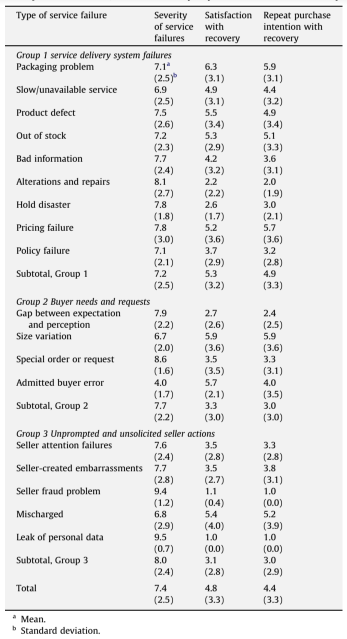
\includegraphics[height=.5\textheight]{images/bab3/Fatalitas-Kegagalan-Ecommerce.png}
        \caption{Fatalitas kegagalan dalam aplikasi Lelang Online, Kepuasan terhadap Perbaikan Pelayanan dan \textit{Repeat Purchase Intention} setelah Perbaikan Layanan}
        \label{severity-failures}
      \end{figure}
      
      \indent Dalam gambar diatas, dijabarkan beberapa jenis kegagalan yang pernah dialami oleh pengguna aplikasi serta fatalitas/pengaruh buruk kegagalan tersebut terhadap kepercayaan pengguna. 
      
	  \begin{figure}[H]
        \centering
        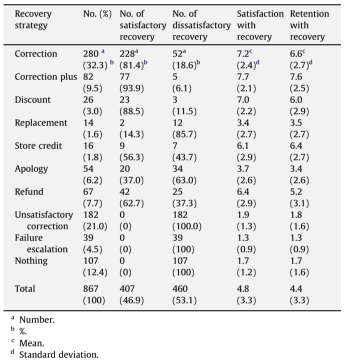
\includegraphics[width=\linewidth]{images/bab3/Solusi-Perbaikan-Ketidakpuasan.png}
        \caption{Kategori Perbaikan terhadap Kegagalan Pelayanan Lelang Online}
        \label{service-recovery-strategies}
      \end{figure}
      
      \indent Maka berdasarkan hasil analisa tersebut, fitur-fitur yang perlu ditambahkan selain daripada fitur dasar aplikasi lelang online adalah sebagai berikut :
      \begin{enumerate}
      \item Fitur chatting, untuk mengurangi kemungkinan \textit{Bad Information} dimana ekspektasi dan persepsi terhadap barang yang dilelang antara pembeli dan penjual tidak sama dan \textit{Special Needs}, 
      \item Fitur pemberian kupon voucher (\textit{Discount and Correction Plus}) yang bisa berupa \textit{free shipping} atau \textit{discount}.
      \end{enumerate}
   %checked
	
	\subsection{\textit{Bussiness Aspects of Software Engineering}}
	
	Lelang merupakan salah satu metode pertukaran barang dan jasa dengan metode penetapan harga yang berbeda dengan perdagangan. Oleh karena itu, lelang juga termasuk dalam kategori bisnis. Yang menarik adalah, ketika bisnis digabungkan dengan teknologi atau yang sering disebut \textit{e-commerce}, hal yang sekedar pertukaran barang bertransformasi menjadi sebuah sistem interaktif yang kompleks dimana tujuan utamanya adalah menarik pengunjung/pengguna untuk menyelesaikan sebuah transaksi. Hal ini tentu sangat krusial, penting, dan tertantang untuk menyelesaikannya. \\
	\indent Dalam mencapai kesuksesan dan tingkat kompetitif yang tinggi, haruslah menyediakan layanan dengan kesan \textit{user experience (UX)} yang positif bagi para penggunanya. Morville  \cite[p.~27]{a-set-of-heuristics-2014} , dalam studi yang dilakukannya, menyebutkan bahwa UX tercakup dalam 7 aspek esensial, yaitu \begin{enumerate}[label=\alph*.]
		\item \textit{useful}
		\item \textit{usable}
		\item \textit{findable}
		\item \textit{desirable}
		\item \textit{accessible}
		\item \textit{credible}.
		\end{enumerate}
	
	\indent Hasil-hasil temuan penting yang menarik dalam pengaruh \textit{user experience}, adalah sebagai berikut dikutip dari sebuah sumber adalah sebagai berikut:
	\begin{enumerate}[label=\alph*.]
		\item \textit{User tend to leave if a page loads more than 3 seconds};
		\item \textit{79\% of users won't return if the web's performance and experience is poor};
		\item \textit{44\% of users will tell the poor experiences to their friends}.
	\end{enumerate}
	
	\indent Selain dari faktor \textit{user experience} dan \textit{performance}, beberapa hal yang menjadi poin penting dan menarik dalam beberapa studi yang terkait adalah sebagai berikut:
	\begin{enumerate}[label=\alph*]
		\item \textit{Familiarity} - yang dapat didefinisikan sebagai tingkat familier atau kesamaan dengan sistem sejenis ternyata dapat membangun \textit{trust} sehingga mensugesti pengguna untuk menyelesaikan transaksi yang dilakukan;
		\item \textit{Usability} yang memudahkan pengguna dalam menyelesaikan transaksi; dan
		\item Aspek-aspek psikologi seperti pemilihan warna, penggunaan \textit{icon} yang sesuai, seperti \textit{icon} gembok pada halaman pembayaran ternyata dapat mengesankan \textit{security} pada pengguna.
	\end{enumerate}
	
	
	\begin{figure}[H]
		\centering
		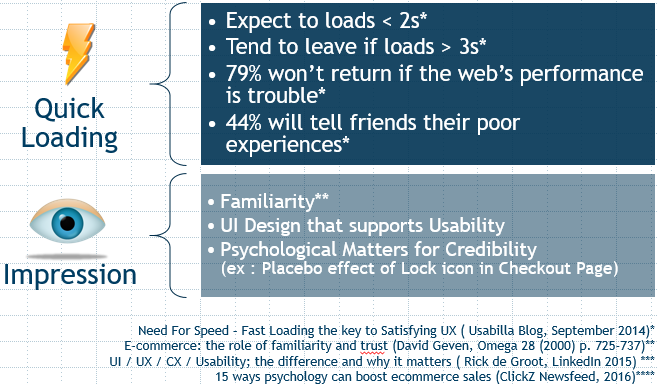
\includegraphics
		[width=\textwidth]
		{images/bab3/analisa/user-centered.png}
		\caption{Visualisasi aspek bisnis dalam \textit{software engineering}}
		\label{user-centered-analysis}
	\end{figure}
	
	\indent Dari hasil temuan ini, dapat disimpulkan bahwa \textit{user experiences, performances, usability} dan psikologi memiliki pengaruh besar dalam kesuksesan lelang online dalam menarik hati para penggunanya. Hal ini akan mempengaruhi definisi kebutuhan fungsionalitas yang akan dibahas dalam subbab \ref{keb-fungsional}.
		
		
		 %checked
	
	\subsection{\textit{Technical Analysis}}
	\label{tech-analysis}
	
	Untuk membuat sebuah aplikasi yang sukses, tentunya banyak sekali aspek yang harus diperhatikan. Selain kualitas aplikasi yang akan dibuat, juga ketahanannya terhadap perubahan karena \textit{e-commerce} adalah sesuatu yang sangat cepat berubah karena kompetitor yang sangat kompetitif dan dorongan tehnologi yang membuat efektifitas dan efisiensi menjadi lebih baik.\\
	
	\indent Dari aspek \textit{software engineering} sendiri, \textit{software engineering} dimaksudkan untuk menunjang/\textit{support} pengembangan \textit{software} daripada \textit{individual programming}. Hal ini mencakup: \begin{inlinelist}
		\item \textit{evolution}
		\item \textit{design}
		\item \textit{supporting program specification}
	\end{inlinelist} \cite{software-engineering}
	
	\begin{figure}[H]
		\centering
		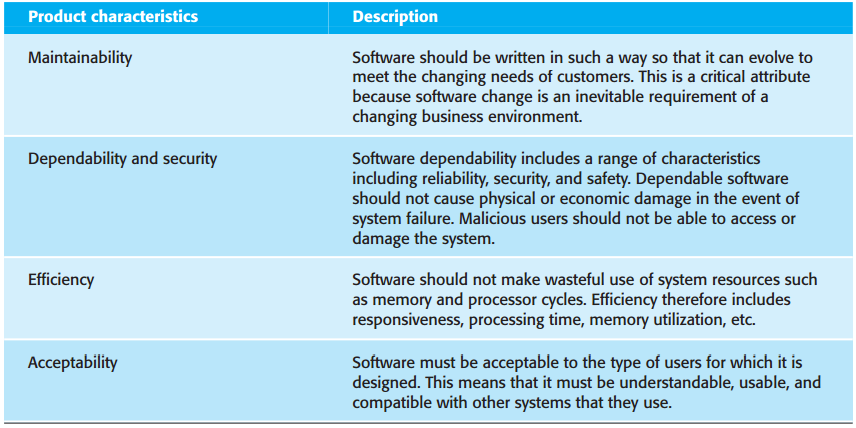
\includegraphics[width=\textwidth]{images/bab3/buku/essential-good-software.png}
		\caption{\textit{Essential attributes of good software}}
		\label{essential-software}
	\end{figure}
	
	\indent Berdasarkan kriteria tersebut, maka setiap poin perlu diperhatikan agar dapat mengembangkan sebuah aplikasi yang tidak hanya sukses, tapi juga bertahan dalam kompetisi. Dalam istilah bisnis, hal ini disebut dengan \textit{risk management \& planning}.
	

 %checked
	
	% pemaparan evolution-risk from inside : data growth, latency
	
	% pemaparan evolution-risk from outside : keamanan
	% pemaparan gabungan 	
	
\subsection{Analisa Penulis}
	\subsubsection{Analisa \textit{User Experience} dari E-Commerce di Indonesia}
	\label{alasan-ux-ecommerce-indonesia alasan-app-serupa}
	Selama masa pengerjaan aplikasi, penulis sering menganalisa dan memperhatikan kebiasaan-kebiasaan yang umum di website \textit{e-commerce} di Indonesia. Salah satu yang paling sering dianalisa oleh penulis adalah adalah situs Tokopedia. Dalam pengembangannya, \textit{user interface} aplikasi akan dipengaruhi analisa ini, yang dijabarkan seperti berikut:
	\begin{enumerate}
		\item Halaman yang muncul bukanlah eagerloading, tapi \textit{lazy loading}\\
		\indent Ini adalah solusi cerdas untuk mengakali \textit{delay loading item} yang sudah pasti jumlahnya sangat banyak (maka butuh \textit{query} yang tentunya memakan waktu cukup lama), namun juga memainkan faktor psikologi / \textit{user behaviour} pengguna dengan membiarkan pengguna melihat tahap demi tahap halaman 'diisi'.
		\item \textit{User Interface} yang sederhana dan pemilihan warna yang \textit{soft}
	\end{enumerate}
	
	\subsubsection{Analisa Keamanan pada koneksi Soket}
	\label{alasan-socket.io}
	Untuk mengakomodasi fitur yang bersifat \textit{realtime}, dibutuhkan koneksi ke soket secara terus menerus. Hal ini tentu dapat menjadi sasaran empuk \textit{security} karena jika tidak diamankan, maka dapat menjadi peluang besar bagi para pihak yang tidak berkepentingan untuk merusak proses bisnis aplikasi.\\
	\indent Namun, jika dalam setiap koneksi soket harus mengirimkan \textit{credentials}, hal ini tentu menjadi tidak praktis dan malah lebih berbahaya karena membiarkan data-data sensitif seperti \textit{password} dan \textit{username} berlalu-lalang di jaringan internet. Selain itu, \textit{disadvantage}nya adalah ketidakpraktisan untuk selalu meng\textit{query} database setiap kali ada koneksi, tentu saja ini memperlambat kerja \textit{database} dan menambah waktu \textit{delay}. Maka dari itu, penulis mengidentifikasi poin-poin penting berikut :
		\begin{itemize}
			\item Hindari \textit{query} database untuk \textit{autentikasi} yang sifatnya masif
			\item Menggunakan mekanisme authentikasi yang menggunakan \textit{credentials} karena rentan dengan masalah keamanan
			\item Mencari metode yang lebih efektif, cepat untuk autentikasi selain 
		\end{itemize}
	
	\subsubsection{Analisa \textit{Best Practice} dalam Struktur Perangkat Lunak}
		\label{alasan-best-practice}
		Pada dasarnya, Laravel adalah kerangka kerja MVC. Namun, ada banyak fitur yang ada dalam aplikasi Lelang Online ini yang tidak terakomodasi dalam MVC, misal sebagai berikut :
		\begin{enumerate}
			\item Sistem Verifikasi lewat Email - yang berarti aplikasi harus berinteraksi dengan SMTP server
			\item Sistem \textit{Generate} Token JWT.io, dimana dalam proses \textit{Generate Token} sama sekali tidak ada database dilibatkan.
		\end{enumerate}
		\indent Jika fitur-fitur tersebut 'dipaksa' dimuat ke dalam MVC, maka tentu saja strukturnya menjadi ganjil, dan muncul \textit{code smell} berikut :
		\begin{enumerate}
			\item \textit{Large Class}, dimana terdapat satu buah file yang sangat panjang (biasanya merupakan entitas utama, dalam hal ini contohnya barang/\textit{item})
			\item \textit{Inappropriate Intimacy}, dimana terdapat satu kelas yang menyimpan \textit{logic} yang tidak seharusnya ia simpan
			\item \textit{Duplicated Code}
		\end{enumerate}		
		\indent Dari hasil analisa ini, penulis mengidentifikasikan strategi-strategi yang akan diterapkan dalam rancangan struktur aplikasi pada subbab \ref{software-structure}, yaitu sebagai berikut:
			\begin{enumerate}
				\item Penggunaan Repository Pattern
				\\ Memisahkan antara Data Processing Layer dan View Layer - agar lebih rapi, terstruktur, hal ini juga dapat menghindari \textit{Duplicated Code}.
				\item Penambahan Komponen : Service dan Provider \\
				Untuk memisahkan \textit{logic} aplikasi yang terkait dengan akses\textit{eksternal services}. Tujuannya, agar jika kedepannya terdapat perbaikan fitur/penambahan fitur, lebih mudah melakukan \textit{traceback} terhadap file/kelas yang bertanggungjawab terhadap fitur tersebut.
			\end{enumerate}
	
	\subsubsection{Analisa Aplikasi Serupa}
	\label{alasan-app-serupa}
		Selama pengerjaan aplikasi, penulis menganalisa aplikasi serupa. Penulis menemukan aplikasi yang kurang lebih alur bisnis/alur penggunaan aplikasinya serupa yaitu : Carousell. Penulis melihat beberapa kesamaan antara sifat transaksi aplikasi tugas akhir saya dengan aplikasi tersebut, yaitu:
		\begin{enumerate}
			\item Sama-sama tidak mengakomodasi pembayaran
			\item Sama-sama tidak adanya kepastian harga (bedanya, pada Carousell yang terjadi adalah \textit{bargaining}
		\end{enumerate} \
		\indent Sehingga dalam alur proses nya, banyak diadaptasi dari Carousell, agar pengguna dapat lebih familiar dan \textit{predictability}nya lebih tinggi jika diadaptasi dari \textit{E-commerce} lainnya yang lebih umum digunakan oleh pengguna.
		
	
	\subsubsection{Analisa Aplikasi Serupa}
	\label{alasan-app-serupa}
	Selama pengerjaan aplikasi, penulis menganalisa aplikasi serupa. Penulis menemukan aplikasi yang kurang lebih alur bisnis / alur penggunaan aplikasinya serupa yaitu : Carousell. \\
	\indent Penulis melihat ada beberapa kesamaan antara sifat transaksi aplikasi tugas akhir saya dengan aplikasi tersebut, yaitu :
	\begin{enumerate}
		\item Sama-sama tidak mengakomodasi pembayaran
		\item Sama-sama tidak adanya kepastian harga (bedanya, pada Carousell yang terjadi adalah \textit{bargaining}
	\end{enumerate}
	\indent Sehingga dalam alur proses nya, banyak diadaptasi dari Carousell, agar pengguna dapat lebih familiar dan \textit{predictability}nya lebih tinggi jika diadaptasi dari \textit{E-commerce} lainnya yang lebih umum digunakan oleh pengguna.
	
	\subsubsection{Analisa Penyimpanan Data}
	
	Untuk penyimpanan data, terdapat 2 jenis data yang sifatnya cukup berbeda, yaitu sebagai berikut:
	\begin{enumerate}
		\item \textbf{Data transaksional disimpan di DBMS SQL - \textit{Relational}}
		\newline
		\indent Data yang sifatnya \textit{transaksional}, seperti data \textit{bidding}, data pengguna, dan lain sebagainya.
		Untuk data ini, lebih baik jika menggunakan database Postgre, untuk menjaga integritas data dan \textit{integrity checking} juga  menjadi lebih baik.
		\item \textbf{Data non-transaksional disimpan di DBMS NoSQL}
		\newline
		\indent Data \textit{chatting}, data \textit{joined rooms} kurang tepat jika disimpan dalam database transaksional karena sifat pertambahan datanya yang sangat cepat, masif dan urgensi integritas data tidak terlalu diprioritaskan (dibanding dengan data transaksional pada poin sebelumnya). Oleh karena itu, baiknya data ini disimpan pada database NoSQL dengan alasan-alasan sebagai berikut.
		\begin{itemize} 
			\item Banyaknya transaksi \textit{read write};
			\item Ketidaksamaan frekuensi \textit{read and write} data semua pengguna;
			\item Sifat permintaan transaksi yang cepat; dan
			\item Kemungkinan perubahan struktur atribut pada pesan (misal: \textit{attachments}, \textit{forwarding}, \textit{replying}, dll) akan sangat menyulitkan pengembangan selanjutnya jika menggunakan database transaksional yang terpaku pada skema database yang ditetapkan di awal pengembangan aplikasi.
		\end{itemize} 	
		
		\item \textbf{Data citra/gambar menggunakan layanan Pihak Ketiga} \newline
		\indent Sekarang telah banyak penyedia jasa \textit{cloud computing} sebagai infrastruktur, seperti Amazon Web Service, Google Cloud Storage Google Alasan-alasan menggunakan AWS sebagai data storage untuk gambar adalah sebagai berikut :
		\begin{enumerate}[noitemsep,topsep=0pt]
			\item Skalabilitas aplikasi lebih terjaga. 
			\newline Dengan memisahkan penyimpanan antara gambar dan server sehingga lebih mudah me\textit{maintain} perkembangan aplikasi, dan lebih fokus terhadap pengembangan aplikasi.
			\item Menyediakan \textit{built-in} keamanan, fleksibel dan efisiensi \cite{wikipedia_amazon_2016}
		\end{enumerate}
		
		\item \textbf{Optimasi \textit{assets}} \newline
		\indent Dalam banyak kesempatan, penulis seringkali mendapati bahwa \textit{delay} untuk \textit{loading assets} lebih lama daripada \textit{loading data} dari database. Berikut penulis akan memaparkan hasil analisa berupa penyebab dan \textit{tackling} permasalahan tersebut.
			\begin{enumerate}
				\item \textit{Useless assets} yang disertakan dalam halaman: Memisahkan \textit{essentials assets} dan menyertakan \textit{script} yang hanya digunakan oleh halaman tersebut.
				\item Logika penyusunan script yang tidak efektif dan optimal (misal: ada satu script yang menyertakan file yang tidak diperlukan): \textit{pre-processing} berupa \textit{minifying, optimization, compiling, compression} terhadap \textit{assets}
				\item Latensi ke \textit{server} yang cukup tinggi (misal: kecepatan sambungan internet yang rendah): \textit{Caching}, \textit{upgrading server} agar dapat "lebih terjangkau" secara jaringan, penerapan PWA (\textit{Progressive Web Apps}) untuk sisi \textit{user experience}.
			\end{enumerate}
	\end{enumerate} %doneded
	
	
	  \subsubsection{Spesifikasi Kebutuhan Fungsional}
  \label{keb-fungsional}
	Berdasarkan deskripsi umum sistem pada subbab \ref{deskripsi-umum-app}, maka dapat disimpulkan bahwa kebutuhan fungsional dari aplikasi lelang online, yang dipaparkan dalam Tabel \ref{tabel-fungsional}.

  \LTXtable{\textwidth}{tables/03b/functional.tex}	
   %checked
	
  \subsection{Spesifikasi Kebutuhan Non-Fungsional}
  
  Kebutuhan non-fungsional yang harus dipeuhi oleh aplikasi ini berhubungan dengan faktor-faktor sebagai berikut:

	\LTXtable{\textwidth}{tables/03b/nonfunctional.tex}	
  
  \newpage %checked
	
	\subsection{Tugas dan Hak Akses Aktor}
	\label{identifikasi_pengguna}

	\indent Aplikasi lelang online dapat digunakan sebagai wadah bagi para pecinta lelang online untuk melakukan kegiatan lelang atau bagi para penjual atau pembeli yang ingin menjual atau membeli barang yang sesuai baik dari kualitas maupun harga. Identifikasi aktor dalam sistem lelang online dijelaskan dalam tabel \ref{identifikasi-aktor}.
	
	\LTXtable{\textwidth}{tables/03/analisa/identifikasi_pengguna}
	
	\LTXtable{\textwidth}{tables/03/analisa/tugas_hak_pengguna}
	
	
	 

	%Technical Analysis